\documentclass[10pt]{beamer}

\usepackage{beamerthemeHannover, graphicx, clrscode, amsmath, amssymb, multicol}
\setbeamercolor{sidebar}{use=structure,bg=gray!20!yellow!80!white}

\title{Solitary Wave Families in Two Non-Integrable Models Using Reversible Systems Theory}
\author[J.A. Leto]{Jonathan Leto}
\date{}

\begin{document}
\frame{\titlepage}

\section{Overview}

\frame{
    \frametitle{Overview}
    \begin{itemize}
    \item Definitions
    \item Background
%    \item Literature Review
%    \item Method of Solution
    \item The Generalized Pochammer-Chree Equations
    \item A Generalized Microstructure Equation
    \end{itemize}
}
\section{Definitions}
\subsection{Reversible System}
\frame{
    \frametitle{Reversible Dynamical System (Iooss \& Adelmeyer)}
    Consider \begin{equation}\label{reversible}
    \frac{dz}{dt} = F\left(z;\mu\right), z \in \mathbb{R}^n, \mu \in \mathbb{R}
    \end{equation} where
    \[F\left(0;0\right)=0\]. 
    If there exists a {\bf unitary map} \[S: \mathbb{R}^n \mapsto \mathbb{R}^n, S \neq I\] such
    that
    \[ F\left(S z; \mu \right) = - S F \left( z;\mu \right) \] for all $z$ and $\mu$
then \eqref{reversible} is a reversible system.
}

\subsection{Solitary Wave}
\frame{
    \frametitle{Families of Solitary Waves}

    Here we will use the term solitary wave or "soliton" to mean a pulse-like solution
    to an evolution equation. For example,
    \begin{equation} A(z) = \ell \mathrm{sech}^2{k z} \end{equation}
    is a two-parameter family of solitary waves.

    where $k$ and $\ell$ are parameters which determine the speed and the height of the wave.
}

%		\begin{center}
%	\includegraphics[width=10cm,bb=0 0 1530 666]{ocb1.png}
% ocb1.png: 72dpi, width=40.96cm, height=19.90cm, bb=0 0 1161 564
%	\end{center}

\section{Background}
\subsection{Normal Forms}

\frame
{
    \frametitle{Normal Form Theory}
    After a nonlinear change of variables (Iooss \& Adelmeyer) one may put the Center Manifold into Normal Form. \\
\bigskip
  {\bf{ Two-Dimensional Center Manifold }}
        \begin{itemize}
        \item $\lambda_{1-4} = 0, 0 , \pm \lambda, \lambda \in \mathbb{R} $
        \item $ Y = A \zeta_0 + B \zeta_1 + \Psi(\epsilon, A,B) $
        \end{itemize}
\bigskip
{\bf{   Four-Dimensional Center Manifold }}
        \begin{itemize}
        \item $\lambda_{1-4} = 0, 0 , \pm i \omega, \omega \in \mathbb{R} $
        \item $ Y = A \zeta_0 + B \zeta_1 + C \zeta_+ + \bar{C} \zeta_- + \Psi(\epsilon, A,B,C,\bar{C}) $
        \end{itemize}
\bigskip
    where $\zeta_0, \zeta_1, \zeta_+, \zeta_-$ are eigenvectors of the linearized operator.
}

\subsection{Bilinear Functions}
\frame {
    \frametitle{Properties of Bilinear Functions} 
    A function \[ B : \mathbb{C} x \mathbb{C} \mapsto \mathbb{C} \] satisfying the following axioms
\begin{subequations}
\begin{eqnarray*}
B(x + y,z) &=& B(x,z) + B(y,z) \\
B( \lambda x, y ) &=& \lambda B(x,y) \\
B(x, y+z) &=& B(x,y) + B(x,z) \\
B(x, \lambda y ) &=& \lambda B(x,y) 
\end{eqnarray*}
\end{subequations}
is called { \bf{bilinear} }.

If $B(x,y)$ is bilinear, then $f(y) \equiv  B(y,y)$ 
is invariant under the transformation $y \mapsto -y$
and thus is { \bf{reversible} }.
}


\section{GPC}
\frame
{
  \frametitle{The Generalized Pochammer-Chree Equations}
The Generalized Pochammer-Chree Equations govern the propagation of longitudinal waves in elastic rods.

\begin{itemize}
\item GPC1
\begin{equation}\label{eq:GPC1}
\left( u - u_{xx} \right)_{tt} - \left( a_1 u + a_2 u^2 + a_3 u^3 \right)_{xx} =0  
\end{equation}
\item GPC2
\begin{equation}  \label{eq:GPC2} 
\left( u - u_{xx} \right)_{tt} - \left( a_1 u + a_3 u^3 + a_5 u^5 \right)_{xx} =0
\end{equation}
\end{itemize}
}
\frame{
    \frametitle{Travelling Wave ODE}

Let $ z = x - c t $ and $u(x,t)=\phi(z)$ to reduce \eqref{eq:GPC1} and \eqref{eq:GPC2} to the Travelling Wave ODE

\begin{equation} \label{eq:gpc-ode}
\phi_{zzzz} - q \phi_{zz} + p \phi = \mathcal{N}_{1,2}[\phi]
\end{equation}
where 
\begin{subequations}
\begin{eqnarray*}
p &\equiv& 0\\
q &\equiv& 1 - \frac{a_1}{c^2} 
\end{eqnarray*}
\end{subequations}

\begin{subequations}
\begin{equation}
L_{pq} = \left( 
\begin{array}{cccc}
0&1&0&0\\
q/3&0&1&0\\
0&q/3&0&1\\
q^2 - p &0&q/3&0 \end{array} \right)
 \end{equation}
\begin{eqnarray*}
\mathcal{N}_1\left[\phi\right] &=& - \frac{1}{c^2}\left[  3 a_3 \left( 2 \phi \phi_z^2 + \phi^2 \phi_{zz} \right) + 2 a_2\left( \phi_{zz} \phi_z + \phi_z^2\right) \right] \\
\mathcal{N}_2\left[\phi\right] &=& - \frac{1}{c^2}\left[ 3 a_3 \left( 2 \phi \phi_z^2 + \phi^2 \phi_{zz}\right) + 5 a_5 \left( 4 \phi^3 \phi_z^2 + \phi^4 \phi_{zz} \right) \right]
\end{eqnarray*}
\end{subequations}

}
\frame{
\frametitle{Reversible Form}

Denoting 
$Y=\left<y_1,y_2,y_3,y_4\right>^T=
\left<\phi,\phi_z,\phi_{zz}, \phi_{zzz}\right>^T$
equation \eqref{eq:gpc-ode} can be written 
\begin{equation}
\frac{dY}{dz}= L_{pq} Y - G_{1,2}(Y,Y)
\end{equation}
where
\[ L_{pq} = \left( 
\begin{array}{cccc}
0&1&0&0\\
q/3&0&1&0\\
0&q/3&0&1\\
q^2 - p &0&q/3&0 \end{array} \right)
\]
\[
G_{1,2}(Y,Y) = \left<0,0,0,-\mathcal{N}_{1,2}\left(Y,Y\right)\right>^T
\]
}
\frame{
\frametitle{Near $C_0$: Normal Form }
The eigenvalues are $\lambda_{1,4}=0,0,\pm \lambda$, $\lambda \in \mathbb{R}$, We write the Center Manifold 
\begin{equation}
Y = A \zeta_0 + B \zeta_1 + \Psi(\epsilon,A,B)
\end{equation}
with corresponding normal form
\begin{subequations}\label{eq:c0nf}
\begin{eqnarray}
\frac{dA}{dz} &=& B \label{eq:c0nfa} \\
\frac{dB}{dz} &=& b \epsilon A + \tilde{c} A^2 \label{eq:c0nfb}
\end{eqnarray}
\end{subequations}
where $\epsilon$ measures the perturbation about $C_0$ and 

\begin{subequations}
\begin{eqnarray}
\zeta_0 &=& \left<1,0,-q/3,0\right>^T \\
\zeta_1 &=& \left<0,1,0,-2q/3\right>^T
 \end{eqnarray}
\end{subequations}
How do we determine the coefficients $b$ and $\tilde{c}$ ?
}

\frame{
    \frametitle{ Finding Coefficients Of The Normal Form }
    \framesubtitle{
    \begin{small}
    \begin{verse}
    When you follow two separate chains of thought, Watson,
    you will find some point of intersection which should approximate 
    the truth.  - \textsf{Sir Arthur Conan Doyle}
    \end{verse} 
    \end{small}
    }

By computing $\frac{dY}{dz}$ in two ways and comparing the coefficients of each
term in the normal form, we find systems of equations which determine each coefficient.
For example, to find $\tilde{c}$, we compare $\mathcal{O}(A^2)$ terms.

}

\frame{
\frametitle{ Two Ways to Compute $\frac{dY}{dz}$ }
\begin{columns}[t]
    \begin{column}{5cm}
    {\bf{Method 1}}\\
    \begin{small} 
    Use the Center Manifold \[Y = A \zeta_0 + B \zeta_1 + \Psi(\epsilon,A,B) \] in the
    reversible system
    \[ \frac{dY}{dz} = L_{pq} Y - G_{1,2}(Y,Y) \] and repeatedly use the bilinear
    properties of $G_{1,2}$ to simplify.
    \end{small}
    \end{column}
    \pause
    \begin{column}{5cm}
    {\bf{Method 2}}\\
    \begin{small}
    Differentiate the Center Manifold
\[Y = A \zeta_0 + B \zeta_1 + \Psi(\epsilon,A,B) \]
and use the Normal Form 

\begin{subequations}
\begin{eqnarray*}
\frac{dA}{dz} &=& B \\
\frac{dB}{dz} &=& b \epsilon A + \tilde{c} A^2
\end{eqnarray*}
\end{subequations}
to simplify all derivatives.
    \end{small}
    \end{column}
\end{columns}
where
\[
\Psi(\epsilon,A,B) = \epsilon A \Psi_{10}^1 + \epsilon B \Psi_{01}^1 + A^2 \Psi_{20}^0 + A B \Psi_{11}^0 + B^2 \Psi_{02}^0 + \cdots
\]
}

\frame{
    \frametitle{Finding $\tilde{c}$ }

Matching $\mathcal{O}\left(A^2\right)$ terms in each method gives us the two
systems of equations
    \begin{columns}[t]
    \begin{column}{5cm}
    {\bf{GPC 1}}
    \begin{tiny}
    \[ \tilde{c} \zeta_1 = L_{0q} \Psi_{20}^0 - G_1\left(\zeta_0,\zeta_0\right) \]
\begin{subequations}
\begin{eqnarray*}
0 &=& x_2 \\
\tilde{c} &=& \frac{q}{3} x_1 + x_3 \label{eq:A2coefbgpc1}\\
0 &=& \frac{q}{3} x_2 + x_4 \implies x_4 = 0 \\
-\frac{2q}{3} \tilde{c} &=& \frac{q}{3}\left(\frac{q}{3} x_1 + x_3 \right) + \frac{q}{3 c^2}\left( 3 a_3 + 5 a_5 \right)\\
&=& \frac{q}{3}\tilde{c} + \frac{q}{3 c^2} a_3 
\end{eqnarray*}
\end{subequations}

\[ \implies \tilde{c} = - \frac{a_3}{3 c^2}  \]
    \end{tiny}
    \end{column}
    \pause
    \begin{column}{5cm}
    {\bf{GPC 2}}
    \begin{tiny}
    \[ \tilde{c} \zeta_1 = L_{0q} \Psi_{20}^0 - G_2\left(\zeta_0,\zeta_0\right) \]
\begin{subequations}
\begin{eqnarray*}
0 &=& x_2 \\
\tilde{c} &=& \frac{q}{3} x_1 + x_3 \label{eq:A2coefbgpc2}\\
0 &=& \frac{q}{3} x_2 + x_4 \implies x_4 = 0\\
 -\frac{2q}{3} \tilde{c} &=& \frac{q}{3}\left(\frac{q}{3} x_1 + x_3 \right) + \frac{q}{3 c^2}\left( 3 a_3 + 5 a_5 \right)\\
  &=& \frac{q}{3}\tilde{c} + \frac{q}{3 c^2}\left( 3 a_3 + 5 a_5 \right) 
\end{eqnarray*}
\end{subequations}

\[\implies \tilde{c} = - \frac{1}{3 c^2} \left(3 a_3 + 5 a_5 \right) \]
\end{tiny}
    \end{column}
    \end{columns}
where $\Psi_{20}^0 = \left<x_1,x_2,x_3,x_4\right>^T$.
}
\frame{
    \frametitle{ Normal Form Near $C_0$ }
Therefore the Normal Form near $C_0$ is

\bigskip

\begin{columns}[t]
\begin{column}{5cm}
    {\bf{GPC 1}}\\
    \begin{small}
    \begin{subequations}\label{eq:c0nfgpc1}
    \begin{eqnarray*}
    \frac{dA}{dz} &=& B \\
    \frac{dB}{dz} &=& -\frac{\epsilon}{q} A - \frac{a_3}{ c^2} A^2
    \end{eqnarray*}
    \end{subequations}
    \end{small}
\end{column}
\begin{column}{5cm}
    {\bf{GPC 2}}\\
    \begin{small}
        \begin{subequations}\label{eq:c0nfgpc2}
        \begin{eqnarray*}
        \frac{dA}{dz} &=& B \\
        \frac{dB}{dz} &=& -\frac{\epsilon}{q} A - \frac{1}{3 c^2} \left(3 a_3 + 5 a_5 \right) A^2
        \end{eqnarray*}
        \end{subequations}
    \end{small}
\end{column}
\end{columns}
These equations admit homoclinic solutions near $C_0$ of the form
\[ A(z) = \ell \mathrm{sech}^2\left(k z \right) \]
}

\frame{
    \frametitle{ Finding $k$ and $\ell$ }
    To determine $k$ and $\ell$, we first write the Normal Form as a single second order equation.
    Then we use our expression for $A(z)$ and 
    compare coefficients of $\mathcal{O}\left(\mathrm{sech}^2(k z)\right)$ and 
$\mathcal{O}\left(\mathrm{sech}^4(k z)\right)$ which implies

\bigskip

\begin{columns}[t]
    \begin{column}{5cm}
    \bigskip
    {\bf{GPC 1}}
    \begin{small}
\begin{subequations} 
\begin{eqnarray*}
k &=& \sqrt{\frac{-\epsilon}{4q}}  \\
\ell &=& \frac{ - 3 \epsilon c^2 }{2 q a_3 } 
\end{eqnarray*}
\end{subequations}
\end{small}
    \end{column}
    \begin{column}{5cm}
    \bigskip
    {\bf{GPC 2}}
    \begin{small}
\begin{subequations} 
\begin{eqnarray*}
k &=& \sqrt{\frac{-\epsilon}{4q}} \label{eq:keq} \\
\ell &=& \frac{ - 9 \epsilon c^2 }{2 q \left(3 a_3 + 5 a_5\right) } 
\end{eqnarray*}
\end{subequations}
    \end{small}
    \end{column}
\end{columns}
\bigskip
Hence, since $\epsilon=-p$, solitons of this form exist for $ p=0^+, q>0$, which 
implies $ a_1 < c^2 $.

}


\frame{
\frametitle{Near $C_1$: Normal Form }
The eigenvalues are $\lambda_{1,4}=0,0,\pm i \omega$, $\omega\in \mathbb{R}$, We write the Center Manifold 
\begin{equation}
Y = A \zeta_0 + B \zeta_1 + C \zeta_+ + \bar{C}\zeta_- + \Psi(\epsilon,A,B, C, \bar{C})
\end{equation}
with corresponding normal form
\begin{subequations}
\begin{eqnarray*}
\frac{dA}{dz} &=& B \\
\frac{dB}{dz} &=& \bar{\nu} \epsilon A + b_* A^2  + c_*\|C\|^2 \\
\frac{dC}{dz} &=& i d_0 C + i \bar{\nu}d_1 C + i d_2 A C 
\end{eqnarray*}
\end{subequations}
where the new eigenvectors co-spanning the four-dimensional Center Manifold are
\[ \lambda_\pm = \left< 1, \lambda_\pm, 2 q/3, \lambda_\pm q /3 \right>^T \]
and $ \lambda_\pm = \pm i \sqrt{-q} $, $q<0$.
}

\frame{
    \frametitle{Compute $\frac{dY}{dz}$ by both methods}

Matching the coefficients of  $A^2$, $\epsilon C$ $\|C\|^2$ and
$AC$ in the two separate expressions for $dY/dz$ yields the
following two systems of equations:

\bigskip

\begin{small}
\begin{subequations}
\begin{eqnarray*}
\mathcal{O}(A^2): &		b_* \zeta_1 &= L_{0q} \Psi_{2000}^0 - G_{1,2}(\zeta_0,\zeta_0) \\
\mathcal{O}(\left|C\right|^2):&	c_* \zeta_1 &= L_{0q} \Psi_{0011}^0 -2 G_{1,2}(\zeta_+,\zeta_-) \label{eq:cstar} \\
\mathcal{O}(\epsilon C): &-\frac{i}{q} \left(d_1 \zeta_+ +  d_0 \Psi_{0010}^1\right) &= L_{0q} \Psi_{0010}^1 \\
\mathcal{O}(A C): 	&i d_2 \zeta_+ + i d_0 \Psi_{1010}^0 &= L_{0q} \Psi_{1010}^0 - 2 G_{1,2}(\zeta_0,\zeta_+)  \label{eq:AC}
\end{eqnarray*}
\end{subequations}
\end{small}
}

\frame{
    \frametitle{ Normal Form near $C_1$ : GPC 1}
    The resolution of the preceding equations yields the coefficients in
    the Normal Form for the GPC 1 equation:
\bigskip
    \bigskip
\begin{subequations}
\begin{eqnarray*}
\frac{dA}{dz} &=& B \\ 
\frac{dB}{dz} &=& -\frac{\epsilon}{q} A + \frac{a_3}{c^2} A^2 + \frac{1}{c^2}\left( \frac{7}{2 \sqrt{-q} } a_3 - \frac{i}{3} a_2 \right)  \left|C\right|^2  \\
\frac{dC}{dz} &=& i \sqrt{-q} C - i \frac{\sqrt{-q} }{q^3} C\epsilon + i \frac{1}{c^2}\left( \frac{7}{2 \sqrt{-q} } a_3 - \frac{i}{3} a_2 \right)A C
\end{eqnarray*}
\end{subequations}
\bigskip
where $ q \equiv 1 - \frac{a_1}{c^2} $
}
\frame{
    \frametitle{ Normal Form near $C_1$: GPC 2 }
    The resolution of the preceding equations yields the coefficients in
    the Normal Form for the GPC 2 equation:
    \bigskip
        \begin{subequations}
        \begin{eqnarray*} 
        \frac{dA}{dz} &=& B \\ 
        \frac{dB}{dz} &=& -\frac{\epsilon}{q} A + \frac{1}{3c^2}\left(3a_3 + 5a_5\right) A^2 + \frac{1}{c^2}\left( 16 a_3 + \frac{140}{3} a_5 \right)  \left|C\right|^2  \\
        \frac{dC}{dz} &=& i \sqrt{-q} C - i \frac{\sqrt{-q} }{q^3} C\epsilon + i \frac{1}{\sqrt{-q} c^2}\left( \frac{7}{2 } a_3 + \frac{32}{3} a_5 \right)A C 
        \end{eqnarray*}
        \end{subequations}
\bigskip
where $ q \equiv 1 - \frac{a_1}{c^2} $
}

\frame{
    \frametitle{ Dynamics Near $C_1$ }

    The two first integrals of the four-dimensional Normal Form are
    \[ K = \|C\|^2 \]
    and
    \[ H = B^2 - \frac{2}{3} b_* A^2 - \bar{\nu} A^2 - 2 c_* K A \]
    \bigskip
    In the $(A,B)$ phase plane, the level curve $H=0$ compromises a homoclinic orbit.
    \bigskip
    The intersection of $H=0$ with the $A$ axis occurs for
    \[
A_{\mp} = \frac{3}{4 b_*} \left[ \bar{\nu} \pm \sqrt{ \bar{\nu}^2 + \frac{16 b_* c_* K}{3} } \right]
\]
}

\frame{
    \frametitle{Homoclinic Orbits for Various Values of H}
		\begin{center}
%	\includegraphics[width=10cm,bb=0 0 1530 666]{ocb1.png}
	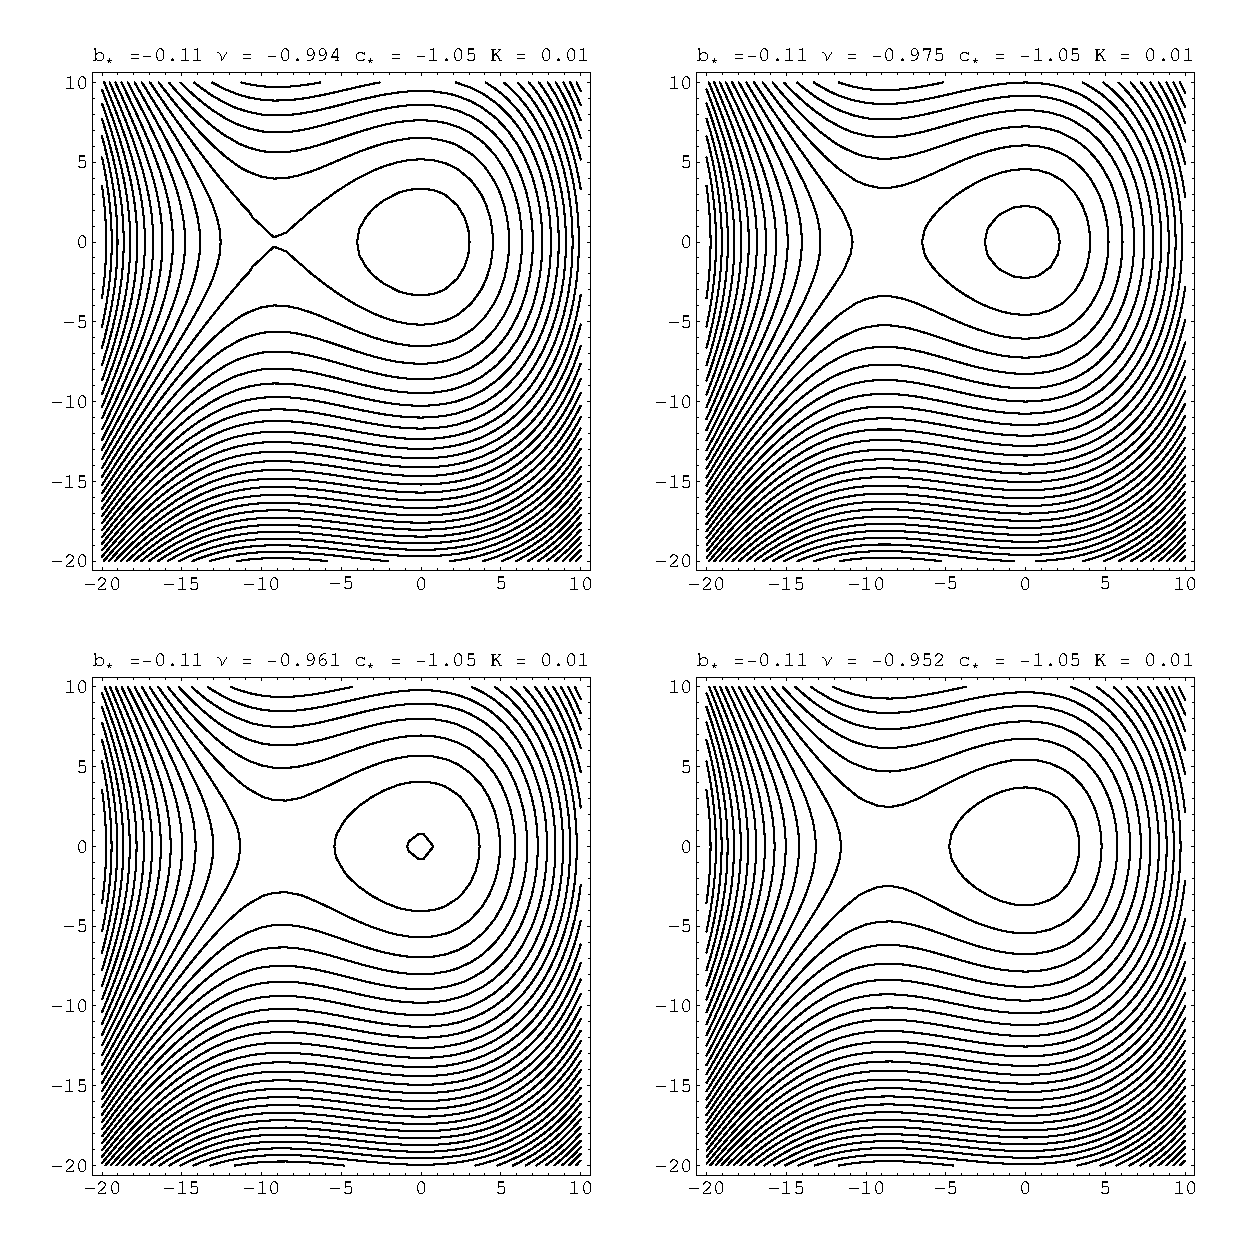
\includegraphics[width=7.42cm, height=7.42cm]{figure2-1c}

	\end{center}
}
\section{MS}
\frame
{
  \frametitle{A Generalized Microstructure PDE}

One dimensional wave propagation in microstructured solids has recently been modeled  by an equation

\begin{equation}\label{eq:MS}
v_{tt} - b v_{xx} - \frac{\mu}{2} \left( v^2 \right)_{xx} - \delta \left( \beta v_{tt} - \gamma v_{xx}\right)_{xx} = 0 
\end{equation}

}
\frame{
    \frametitle{Travelling Wave ODE}

Let $ z = x - c t $ and $u(x,t)=\phi(z)$ to reduce \eqref{eq:MS} to the Travelling Wave ODE

\begin{equation} \label{eq:ms-ode}
\phi_{zzzz} - q \phi_{zz} + p \phi = \mathcal{N}[\phi]
\end{equation}
where 
\begin{equation}
\mathcal{N}\left[\phi\right] = -\Delta_1 \phi_z^2 - b \Delta_1 \phi \phi_{zz}
\end{equation}

\begin{subequations}
\begin{eqnarray*}
z &\equiv& x - c t\\
p &\equiv& 0\label{eq:pdef} \\
q &\equiv & \frac{c^2 - b}{\delta\left(\beta c^2 - \gamma\right)} 
\label{eq:qdef2} \\
\Delta_1 &\equiv& \frac{\mu}{ \delta\left( \beta c^2 - \gamma\right) }\label{eq:deltadef} 
\end{eqnarray*}
\end{subequations}
}

\frame{
    \frametitle{Normal Form near $C_0$}

With the same kind analysis we find

\begin{subequations}
\begin{eqnarray*}
\frac{dA}{dz} &=& B \\
\frac{dB}{dz} &=& -\frac{\epsilon}{q} A - \frac{ b \Delta_1}{3}  A^2
\end{eqnarray*}
\end{subequations}
}

\frame{
    \frametitle{ Solitary Waves Near $C_0$ }

The Normal Form admits a homoclinic solution near $C_0$ of the form

\[A\left(z\right) = \ell \space \mathrm{sech}^2\left(k z\right) \]
\bigskip
where
\bigskip
\begin{subequations}
\begin{eqnarray*}
k &=& \sqrt{\frac{-\epsilon}{4q}}  \\
\ell &=& \frac{6 k^2}{ b \Delta_1 }
 \end{eqnarray*}
\end{subequations}

Since $\epsilon = -p$, and the curve $C_0$ corresponds to $p=0,q>0$, solitary waves
exist near $C_0$ for $p>0, q> 0$, which implies
that $  \frac{c^2 - b}{\delta\left(\beta c^2 - \gamma\right)} > 0 $.
}
\frame{
    \frametitle{Normal Form near $C_1$ }

Near $C_1$ the Normal Form for \eqref{eq:MS} is
\begin{subequations}
\begin{eqnarray*} 
\frac{dA}{dz} &=& B  \\
\frac{dB}{dz} &=& -\frac{\epsilon}{q} A - \frac{b \Delta_1 }{3} A^2 + 2 \Delta_1 \left(\frac{2 b }{3} - 1\right) \left|C\right|^2 \\
\frac{dC}{dz} &=& i \sqrt{-q} C - i \frac{\sqrt{-q} }{q^3} C\epsilon + i \frac{b \Delta_1}{6 \sqrt{-q}} A C 
\end{eqnarray*}
\end{subequations}

}

\frame{
    \frametitle{Homoclinic Orbits for Various Values of H}
		\begin{center}
%	\includegraphics[width=10cm,bb=0 0 1530 666]{ocb1.png}
	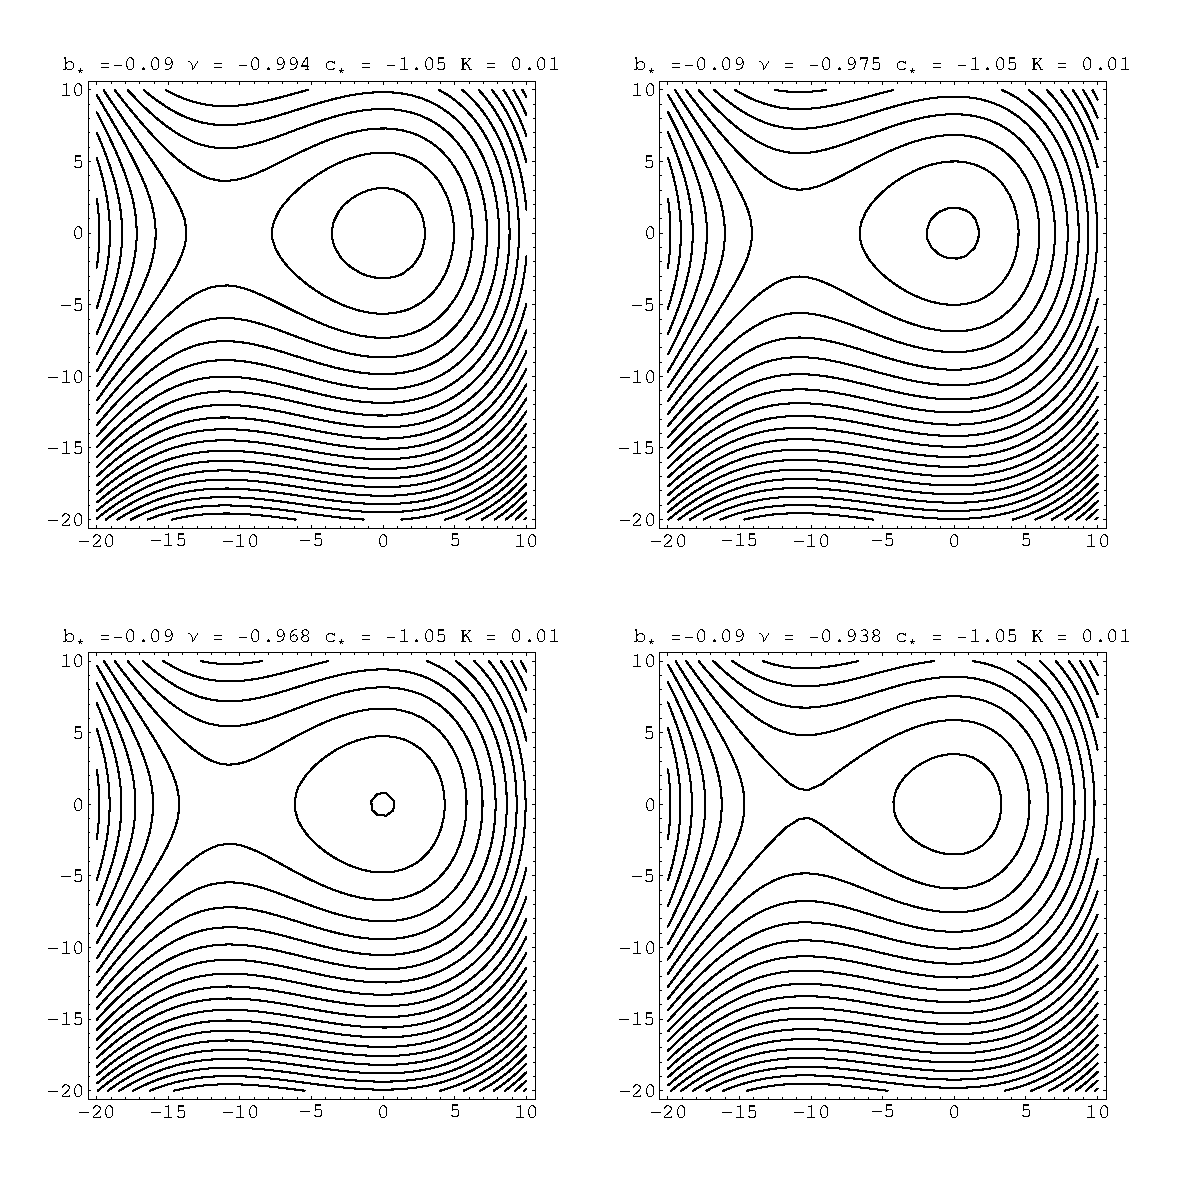
\includegraphics[width=7.42cm, height=7.42cm]{figure3-1a}
	\end{center}
}

\frame{
    \frametitle{Open Problems}

}
\frame{
    \frametitle{Thanks}

    \begin{itemize}
    \item Dr. Choudhury, Dr. Mohapatra, Dr. Rollins for being great committee members
    \item Erin Langsdorf for being my Orlando graduation liason
    \end{itemize}
}
\end{document}
